\documentclass[
	12pt, % Default font size, values between 10pt-12pt are allowed
	%letterpaper, % Uncomment for US letter paper size
	%spanish, % Uncomment for Spanish
]{fphw_assignment_toc}

\usepackage{my_packages}
\usepackage{graphicx}
\usepackage{lipsum}
\usepackage{etoolbox}

%------------------------------------------------------------------------------------


\title{Project report M1:}        % Assignment title
\author{SCHUFFENECKER Antoine}    % Student name
\roll{Intern}                    % Class roll
\class{Master 1 Csmi}              % Class
\session{2020/2021}             % Session
\email{antoine.schuffenecker@gmail.com}
\date{29/05}        % Due date
\institute{}              % Institute or school name
\course{PROJET}                            % Course or course name
\professor{Cristhophe PRUD'HOMME}            % Professor or teacher in charge of the assignment

%------------------------------------------------------------------------------------
\addbibresource{ref.bib} 

\setcounter{secnumdepth}{-2} 
%\renewcommand{\thesection}{}  % https://tex.stackexchange.com/a/30202/114006
%------------------------------------------------------------------------------------
\begin{document}
\maketitle
\pagenumbering{gobble}           % to remove the page numbering
\newpage
\pdfbookmark[section]{\contentsname}{toc}
\tableofcontents
\raggedbottom 
\newpage
\pagenumbering{arabic}          % to start the page numbering

%-----------------------------------------

\section{\large\bf  Introduction~}\vspace{\dimexpr-40pt-\baselineskip+3cm}

\subsubsection{\large\bf1.Context:}\vspace{\dimexpr-40pt-\baselineskip+3cm}

\vspace{\dimexpr-40pt-\baselineskip+3cm}

The sport has a great influence on health, it is shown in many article . For example in the study of the young population in Belgium, it is shown and demonstrated that a healthy and reasonable practice of sports in our daily  life habits reduces the risk of cardiac incident. The earlier these life habits are introduced in the individuals routine the greater the positive impact is. This is a public health organisation problem because like the study mentioned before we can fin other ones which states on the impact of physical activities on risks of diseases such as cancer, diabetes,etc.
\\
Now we want to try to evaluate how the population, in terms of physical abilities, reacted to the Covid-19 which forced a lot of people to stop any sports.
\\
The students of STAPS takes physical tests when they arrive the first year in the cursus. These tests are organised around 4 core notions : Strength, Speed, Coordination and Endurance. The results of these test gives a grade. The common trend is to say that performances are worse every year which might not be true. 

\\ 
However the Covid happened and with it a lot of students could not practice any sport for long periods of time. So we might see an impact on performances.
\\
There is at the moment one data set:

- The whole results of all STAPS students since 1999, roughly 20000 results.


\\
\subsubsection{\large\bf 2.Supervisors:}
\vspace{\dimexpr-40pt-\baselineskip+3cm}

My supervisor is Christophe Schnitzler. Expert in physical mobility, formation of teachers and Education to healthcare by sport.
\\
\\
\\
\subsubsection{\large\bf 3.Subject:}

With the context given we have now 3 major questions :

- How did the overall performances of all students changes during all these years ?

- How exactly did the covid impacted the students on a physical level ?

- Did the covid impacted the students differently regarding their gender ?


\\
\\
\newpage

\section{\large\bf I) Data~}
\subsubsection{\large\bf 1.Presentation: }


Since 1999 the STAPS direction imposes on their students to take the BCPE test which consists of several physical exams to determine the physical shape of their students. These are separated in categories speed, endurance, strength, coordination and others. 
\\
All this data is stored in files. Since some modalities or responsible have changed through the years, the files are not exploitable with no pre-treatments to gather all of it in an efficient way. For example some of the trials have changed to measure with a better accuracy physical qualities. The first batch of data is dated between 1999  and 2015, the second one is 2016,the data from 2017 and 2018 are not exploitable, it is missing way too many results about the exams, then each year  is a single file but has a similar architecture. The data stops in 2021.
\\
There is some precision about the data, on the 1st batch it is an excel file, each sheet represents a year. In 1999 there are no results for mens, and in 2015 the grade of the overall test is missing. 
On the second batch it is a pdf file which needs special treatment.
On the last one it is again different excel files with different sheets but  on the results one are used.

\newpage


\subsubsection{\large\bf 2.Data_Cleaning:}

The main work that I had to do was to clean all the data. My results come from a lot of trials to be sure that every errors and exceptions are treated to obtain a very clean dataframe. Which will be the easiest to use. I will explain all my methodology for each batch.
\\
\bigskip

To obtain useful data we need it to be present in most years with little to no change on the exercises asked to the students so we can see clearly the evolution and the impact of any perturbation like we would like to see.
\\

The list I chose is the following:
\\
\bigskip
\\
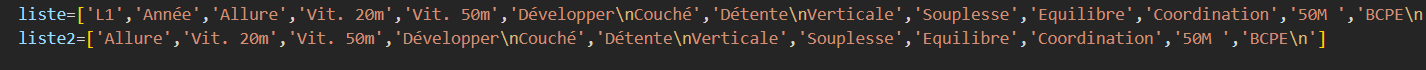
\includegraphics[scale=0.5]{Images/liste.png}
\\
\bigskip
(‘L1’ and ‘Année’ are here to give the gender and the year of the results of a line).

On the first hand for the first batch, I started with moving the following data from excel in a dataframe.
\\
\bigskip
\\
\includegraphics[scale=0.7]{Images/données_excel(1999-2015).png}
\\
\bigskip
\\
\newpage
I had to replace every ‘m’,’g’ and some variations (some with space in it) with ‘M’, which will help later display all the data. The same had to be done for female students but with only variation of ‘f’ replaced by ‘F’. Then since the columns had not the same name through the years I chose the  ones who were used the most recently.
To do so i had to copy the right columns and then select only the ones that will be needed later
\\
\bigskip
\\
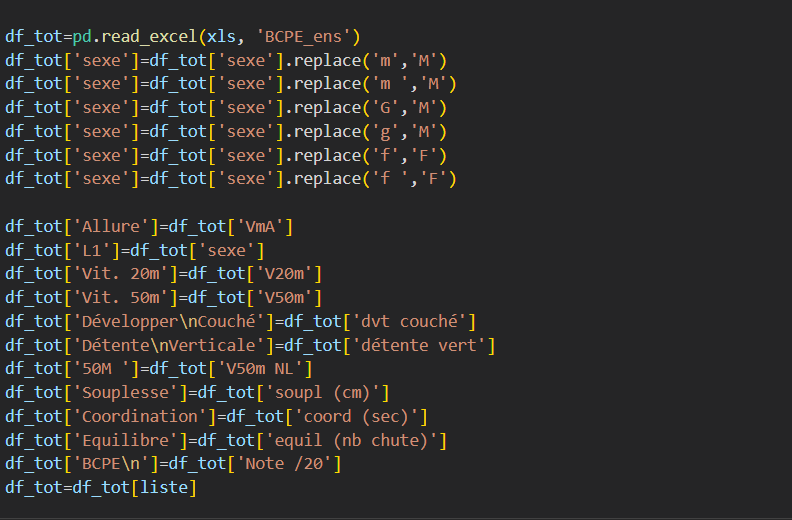
\includegraphics[scale=0.8]{Images/clean_batch_1.png}
\\
\bigskip
\\
Then on the second batch I had to use a different approach because it is a pdf file, the mains issue with the file is that the pdf was not in a exploitable format, I had to search by hand to reassign the right columns to the variable needed. Since the format was not well design a lot of the data was very hard to exploit. It might later gives some issue with the 2016 year. Furthermore the way of writing float number with "," introduced a lot of bugs that I had a hard time to detect.
\\
\bigskip
\\
\includegraphics[scale=0.8]{Images/données_pdf(2016).png}
\\
\bigskip
\\
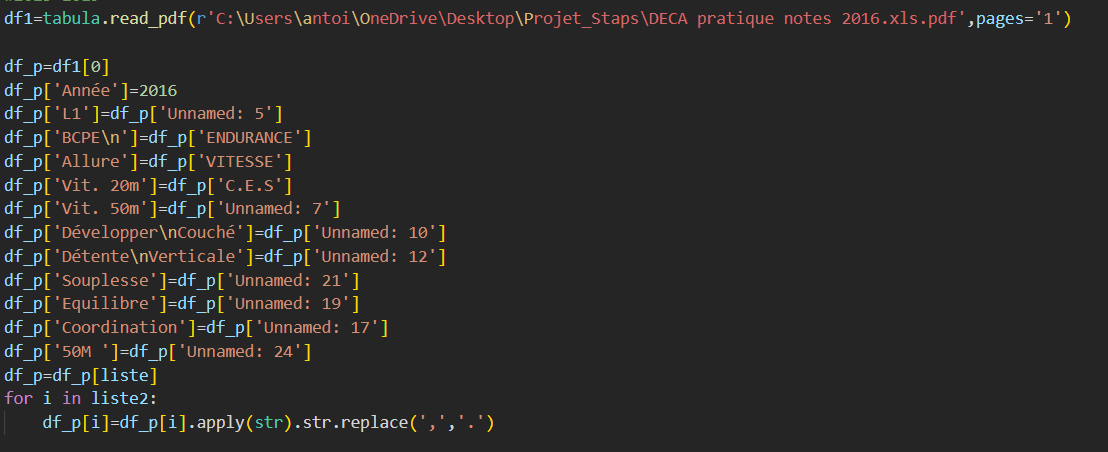
\includegraphics[scale=0.8]{Images/clean_batch_2.png}
\\
\bigskip
\\
\newpage
For the latest batch I tought i would only have to create a a columns 'Année' but an error in the columns of the year 2020 made me redefine all the columns to ensure the right results. I also had to change the 'G' into 'M'. BUt apart from that the data was for the most part much more easier to use ( it has to do with choice i made for the columns names but still a good point).
\\
\bigskip
\\
\includegraphics[scale=0.8]{Images/données_excel(2019).png}
\\
\bigskip
\\
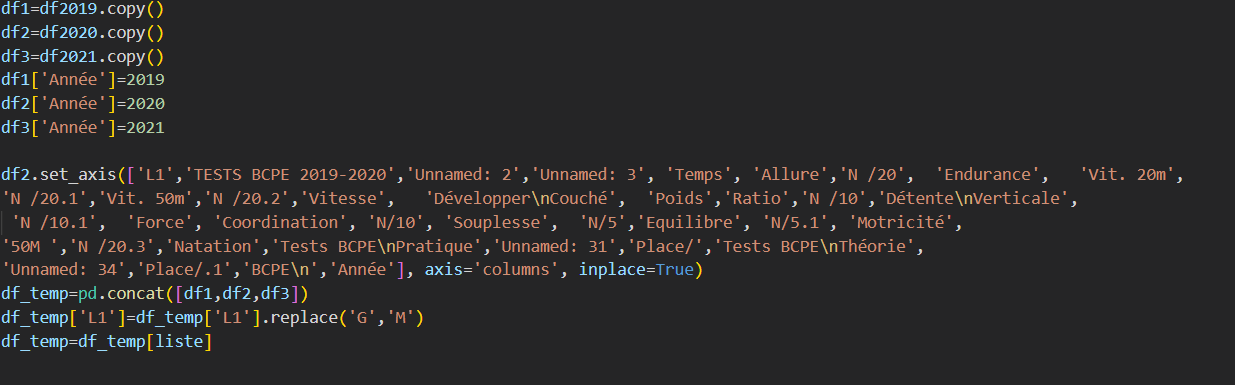
\includegraphics[scale=1]{Images/clean_batch_3.png}
\\
\bigskip
\\
Now we just have to concatenate all these dataframe and we will treat it as a whole.

In the end there are still some rows which are unusable. I thought about which one to exclude, since we only care about the performances and the actual results in each trials any student who was absent to any of them will be discarded, for those who has already take the test any prior year will be also discarded ( to only have one occurrence of those students), finally the one who are dispensed to do the trials are obviously also excluded of the study.
\\
\bigskip
\\
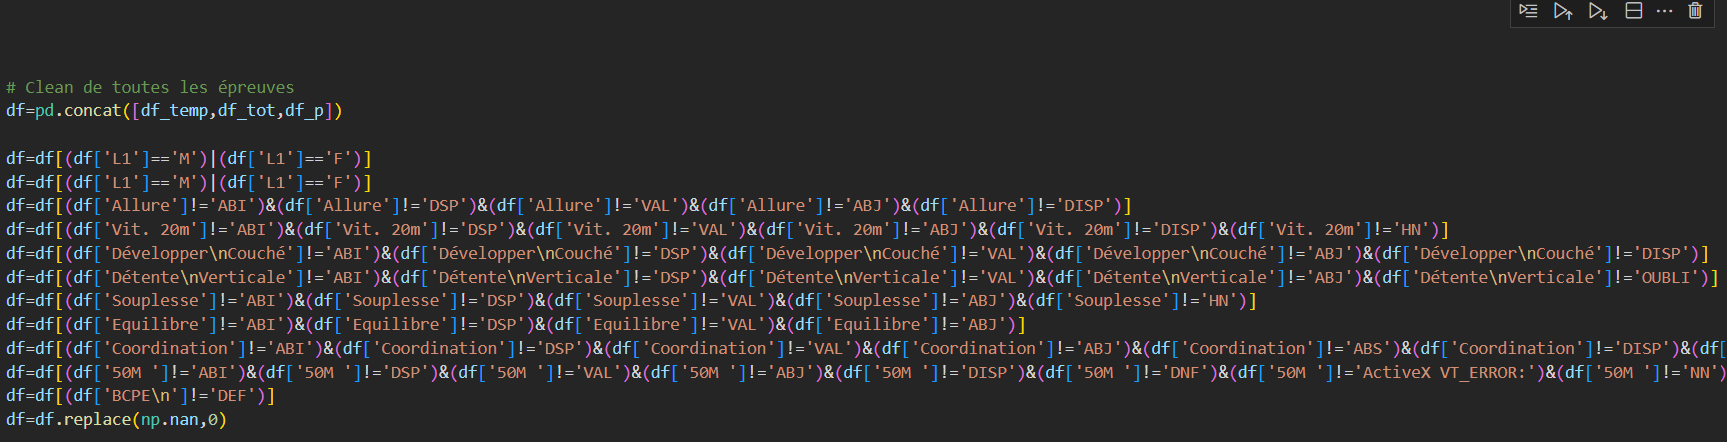
\includegraphics[scale=1]{Images/clean_bool.png}

There is still some actions needed, change the data to be sure all trials over the year are measured with the same units, and exclude any strange rows.
\\
\bigskip
\\
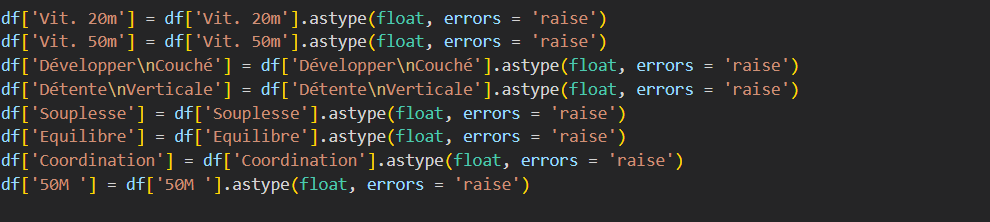
\includegraphics[scale=1]{Images/clean_float.png}


\newpage

\subsubsection{\large\bf 4.Cleaning_result:}

So this is the result that I get 
\\
\bigskip
\\
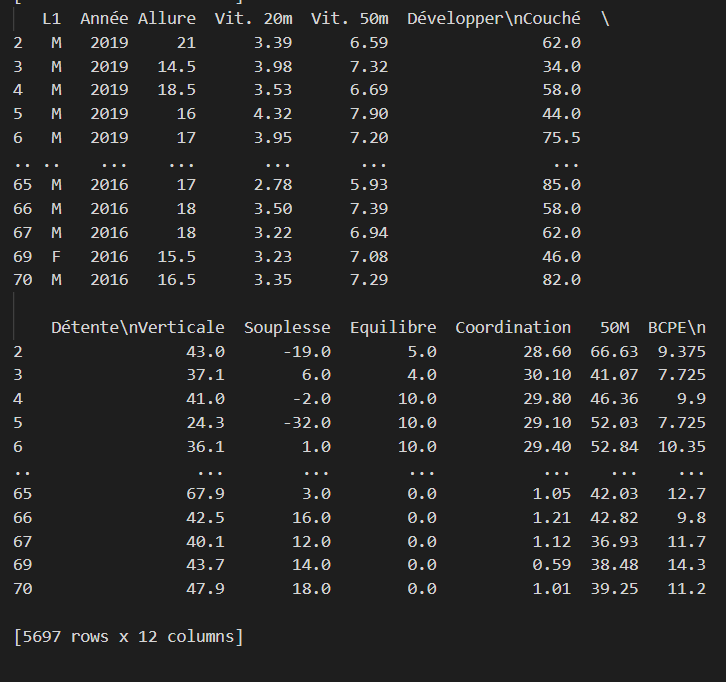
\includegraphics[scale=1]{Images/clean_df.png}
\\
\bigskip
\\
Those results will be stored in a excel file if anybody needs it in the future
\\
\bigskip
\\
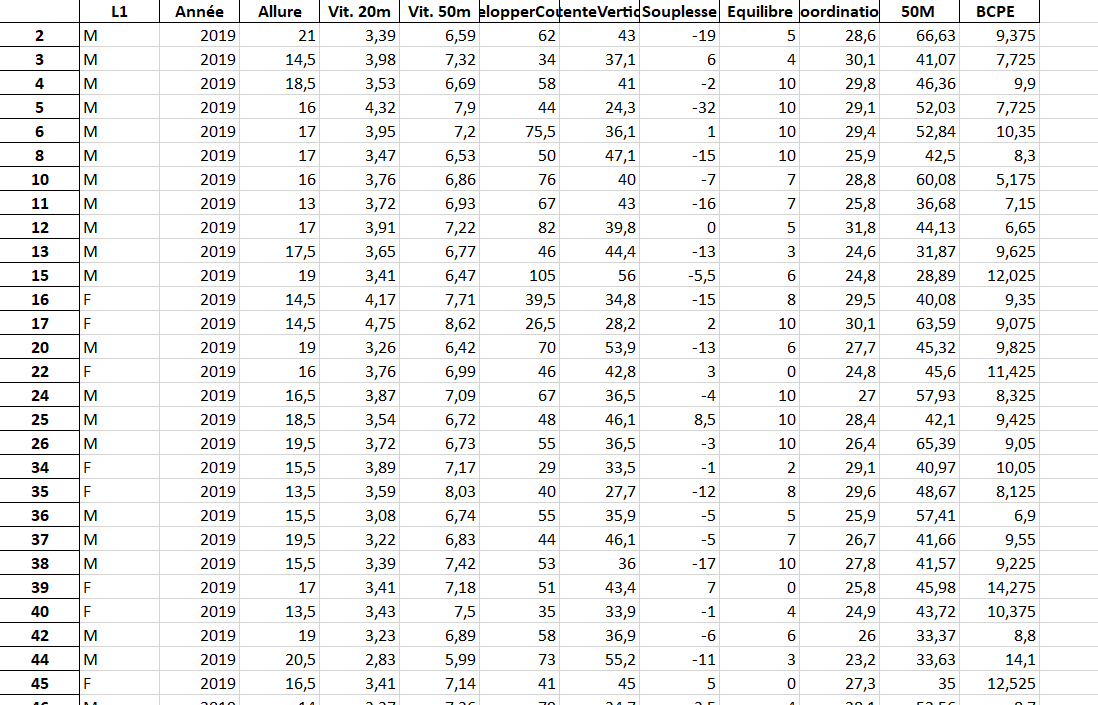
\includegraphics[scale=1]{Images/clean_data_excel.png}
\\
\bigskip
\\
\newpage
\section{\large\bf II) Primary_results~}
\subsubsection{\large\bf 1.Statistics_on_every_elements: }

Now that we have a clean data frame with no issue in it we can obtain some basics stats on it, the mean, the max the min, the standard deviation, the quartile. For every columns of data and either for the whole data or for any years specifically. 

So first there is the stats for the whole data frame.
\\
\bigskip
\\
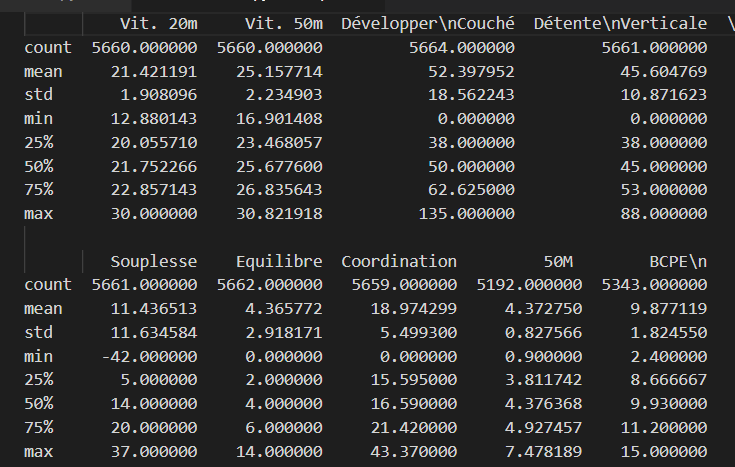
\includegraphics[scale=0.8]{Images/stats.png}
\\
\bigskip
\\
Here i took the example of the year 2005
\\
\bigskip
\\
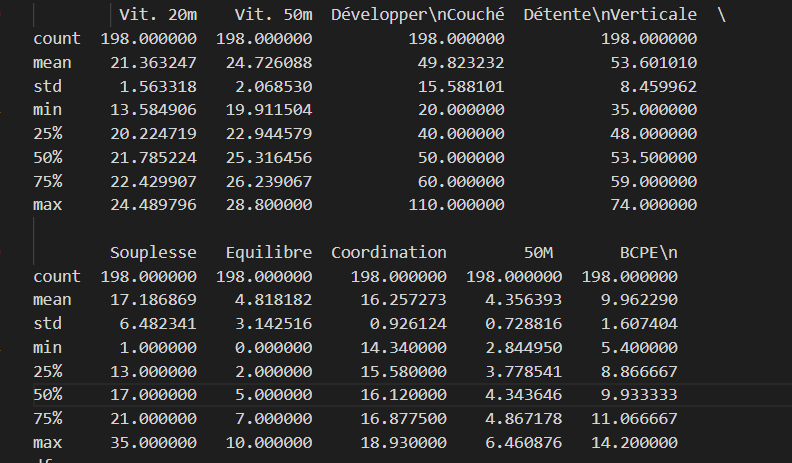
\includegraphics[scale=0.8]{Images/stats2005.png}
\\
\bigskip
\\

\subsubsection{\large\bf 2.Graphs: }

For each variable we choose now we can the see the evolution of the mean during the 20 years span, it will help to decide what are are our hypothesis for the more complex analysis yet to come.

\\
The endurance test with VmA measurements 
\\
\bigskip
\\
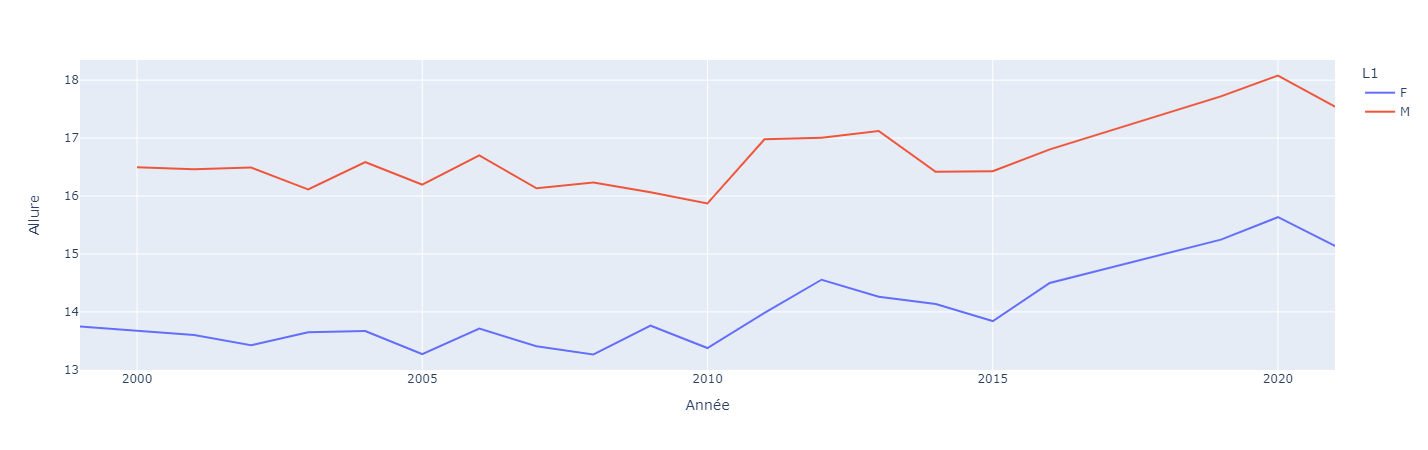
\includegraphics[scale=0.4]{Images/Allure.png}
\\
\bigskip
\\
The speed on 20 meters (in km/h)
\\
\bigskip
\\
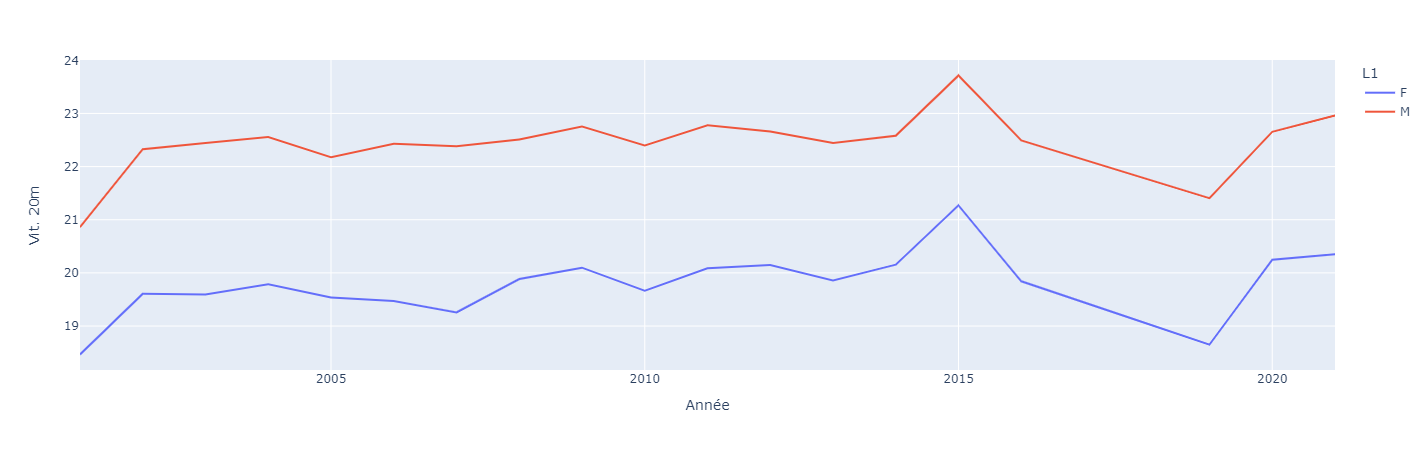
\includegraphics[scale=0.4]{Images/Vit.20m.png}
\\
\bigskip
\\
\newpage
The speed on 50 meters (in km/h)
\\
\bigskip
\\
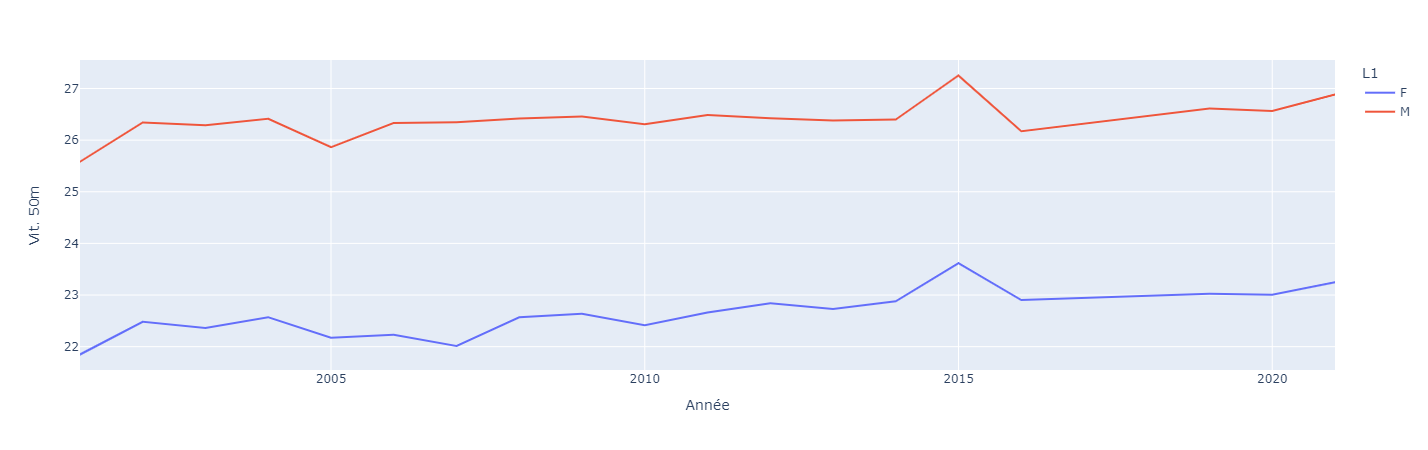
\includegraphics[scale=0.4]{Images/Vit.50m.png}
\\
\bigskip
\\
The bench press (in kg)
\\
\bigskip
\\
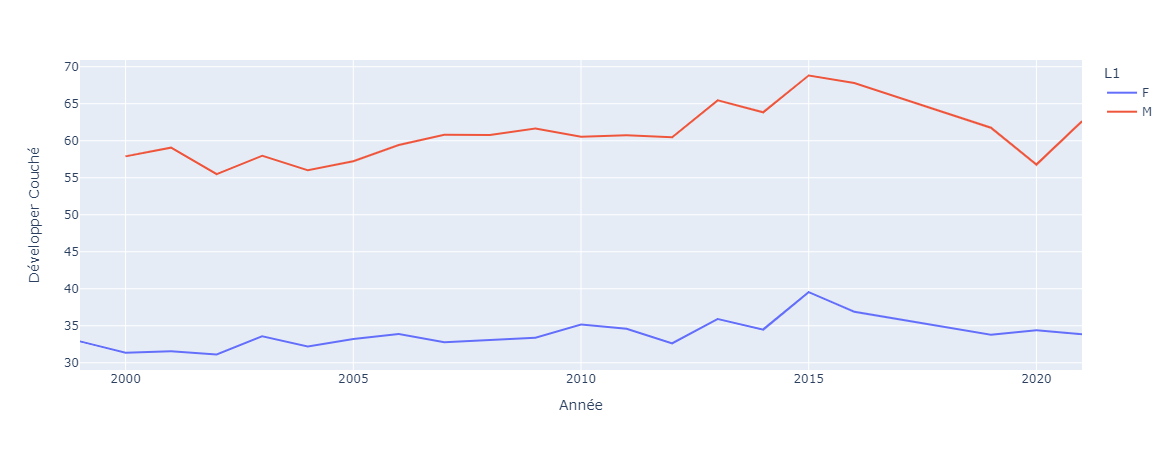
\includegraphics[scale=0.4]{Images/Developpe.png}
\\
\bigskip
\\
The vertical elasticity (in cm)
\\
\bigskip
\\
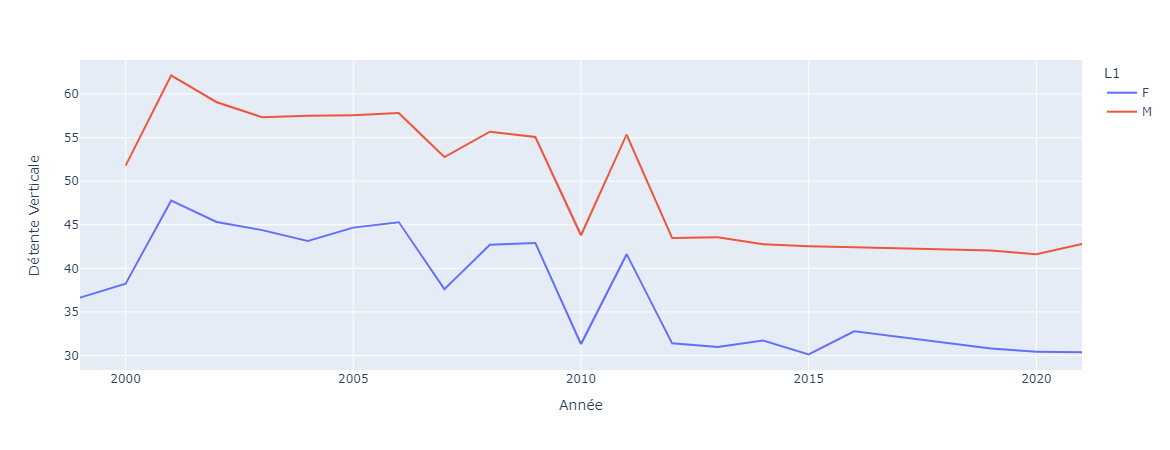
\includegraphics[scale=0.4]{Images/Detente.png}
\\
\bigskip
\\
The flexibility (in cm)
\\
\bigskip
\\
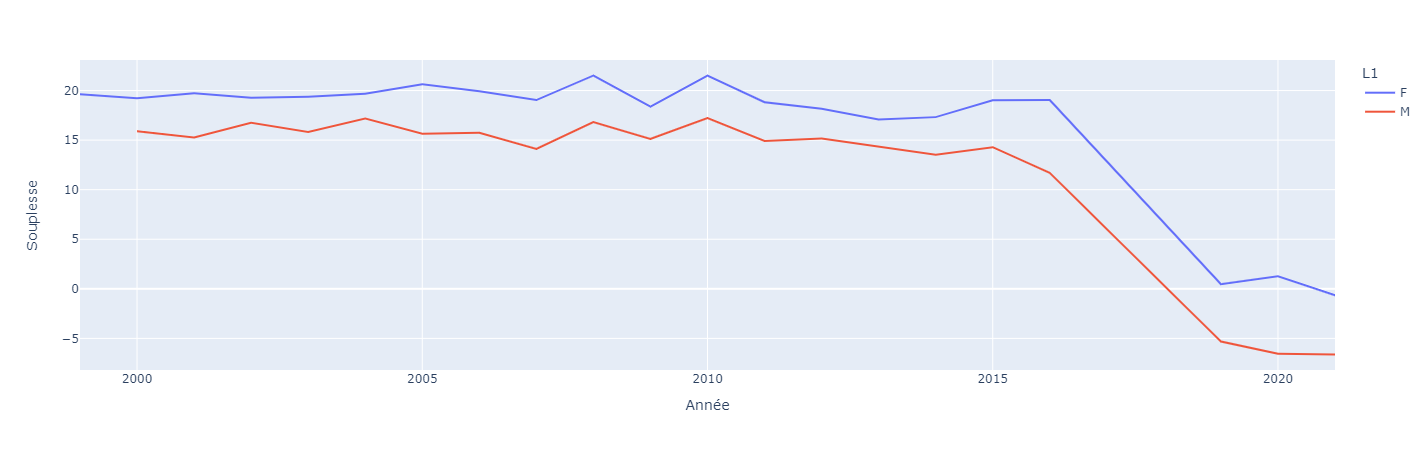
\includegraphics[scale=0.4]{Images/souplesse.png}
\\
\bigskip
\\
The balance ( in number of fall)
\\
\bigskip
\\
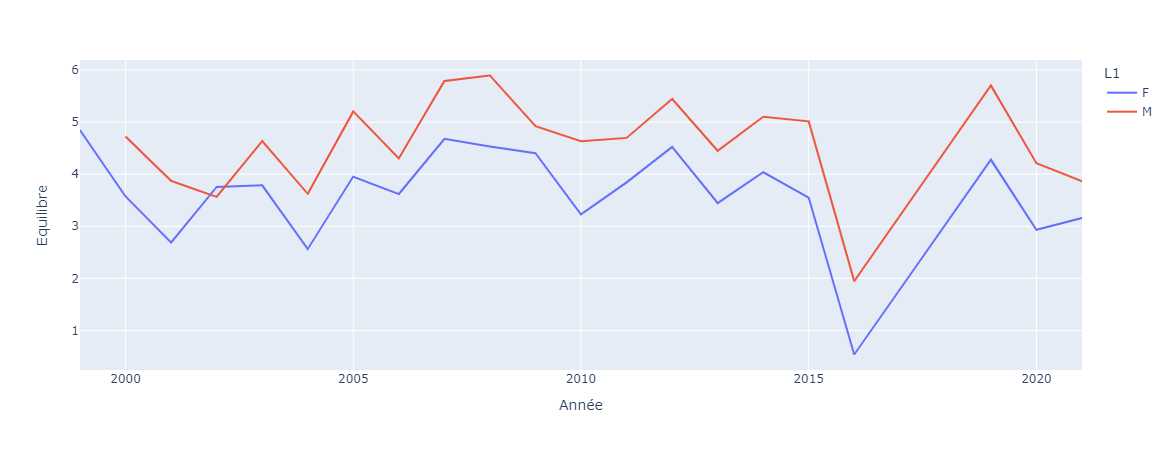
\includegraphics[scale=0.4]{Images/Equilibre.png}
\\
\bigskip
\\
\newpage
The coordination 
\\
\bigskip
\\
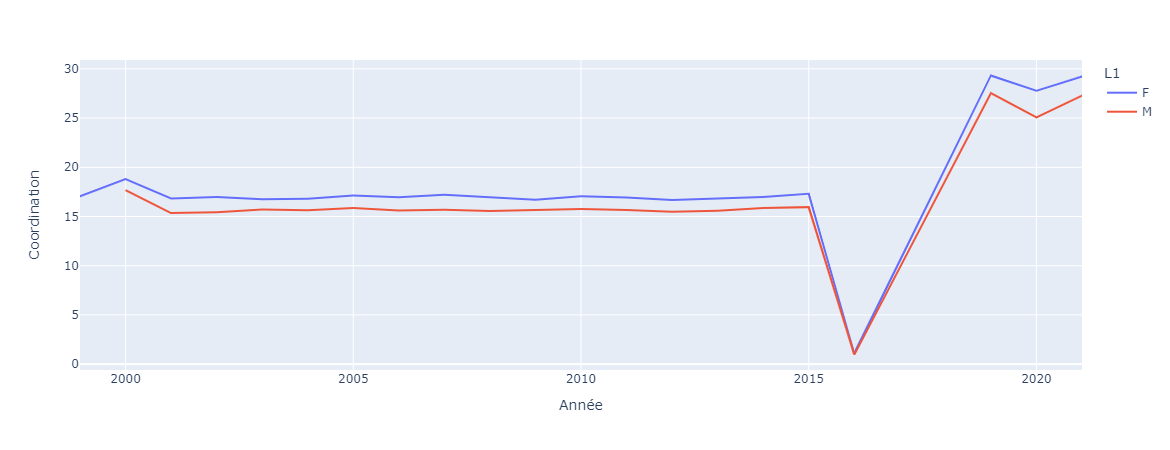
\includegraphics[scale=0.4]{Images/Coordination.png}
\\
\bigskip
\\
The swimming speed  on 50 meters (in km/h)
\\
\bigskip
\\
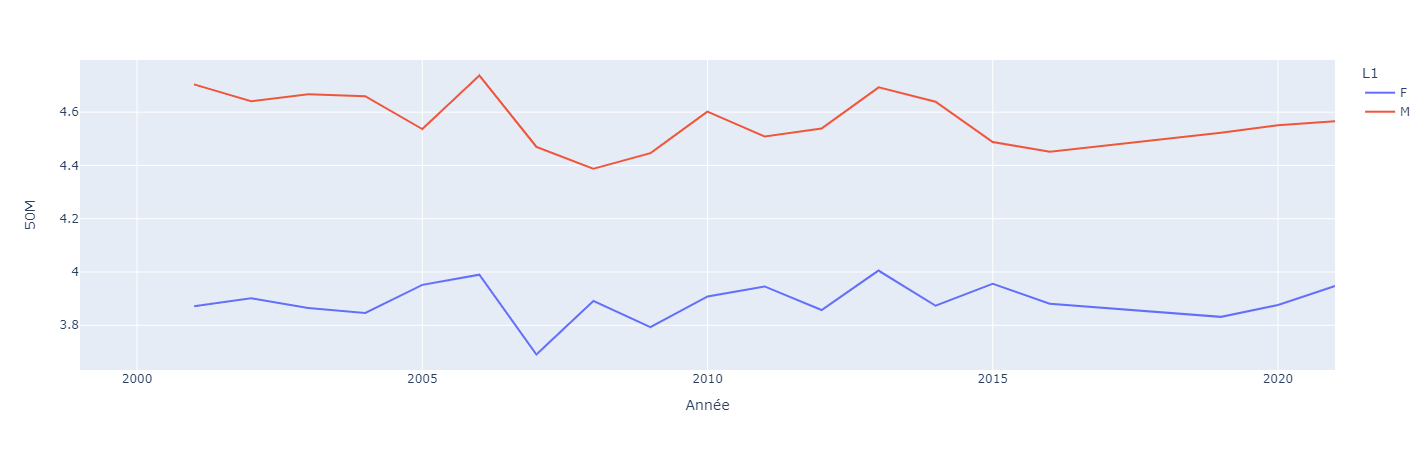
\includegraphics[scale=0.4]{Images/natation.png}
\\
\bigskip
\\
The overall mark on the exam (with the missing data of 2015)
\\
\bigskip
\\
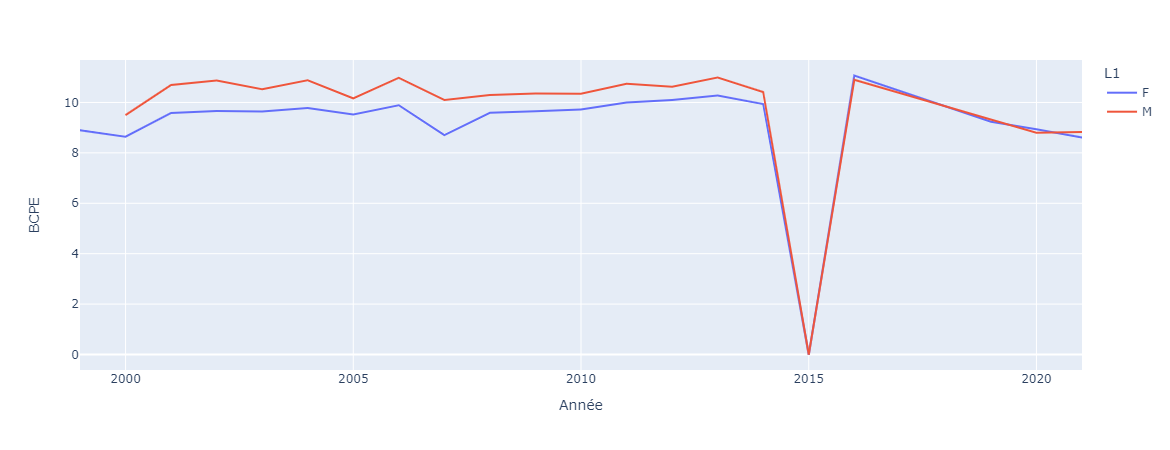
\includegraphics[scale=0.4]{Images/notes.png}
\\
\bigskip
\\

\section{\large\bf III) Advanced results~}

Now that we saw the results of simple stats we can make greater assumptions about the data,depending on which element it is.

\\
The Covid had an impact on the trials:
\\
- Speed on 20 meters.
\\
- The bench press for the men.
\\
- The flexibility.
\\
-The coordination (positive impact)
\\
- The swimming speed on 50 meters.
\\
- The mark of the exam.
\\
\bigskip
\\


The Covid had no impact on :
\\
-The balance.
\\
-Speed on 50 meters.
\\
-Vertical elasticity
\\
-The endurance test
\\


Now we got our hypothesis for our tests and we try to conduct it on 2 of them : the Anova test and the Friedman Anova test. We want to verify the result that we can see on the means graph and the general idea that  we suppose on it. To do so we use the Anova test and in case the Anova test does not conclude due to problems on the value of the data the Friedman anova test.

\newpage

\subsubsection{\large\bf 1.ANOVA: }
\\
To perform an ANOVA we have to check several properties first. 
\\
The fact that the different samples (here the result for each years) are independent, this is obviously the fact because results from on year can not influence one on an other year. 
\\
The equality of the variance (which should be the case because if the distribution of the performances) but we will verify it with a Bartlett test 
\\
The normality of the rest with a Shapiro test.
\\
If these three condition are met the result of the ANOVA will be relevant for our study.
The expected result is to find that the ANOVA says that the means are not the same and then with a some t-tests we would like to see that the covid years are the one which prevent it.
\\
Unfortunately after trying to do the Bartlett test it is shown that the data had way too much disparities in the variance and the test was not conclusive. Because of that the ANOVA test could not be used.
\bigskip
\\
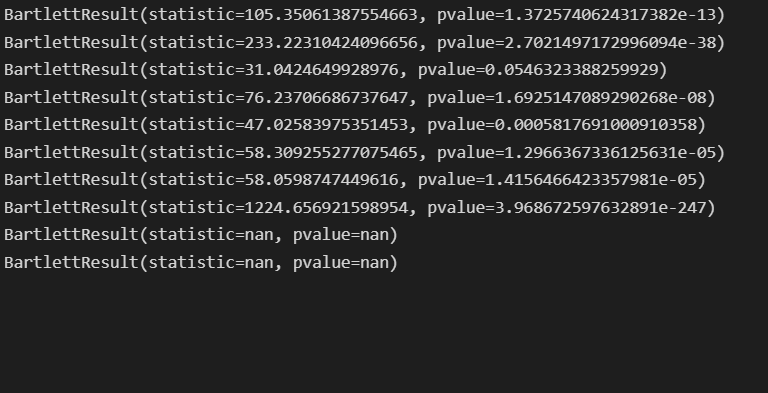
\includegraphics[scale=1]{Images/Bartlett.png}
\\
\bigskip
\\
\newpage
\subsubsection{\large\bf 2.Friedman_ANOVA: }

So now we have to try the Friedmann Anova.
\bigskip
\\
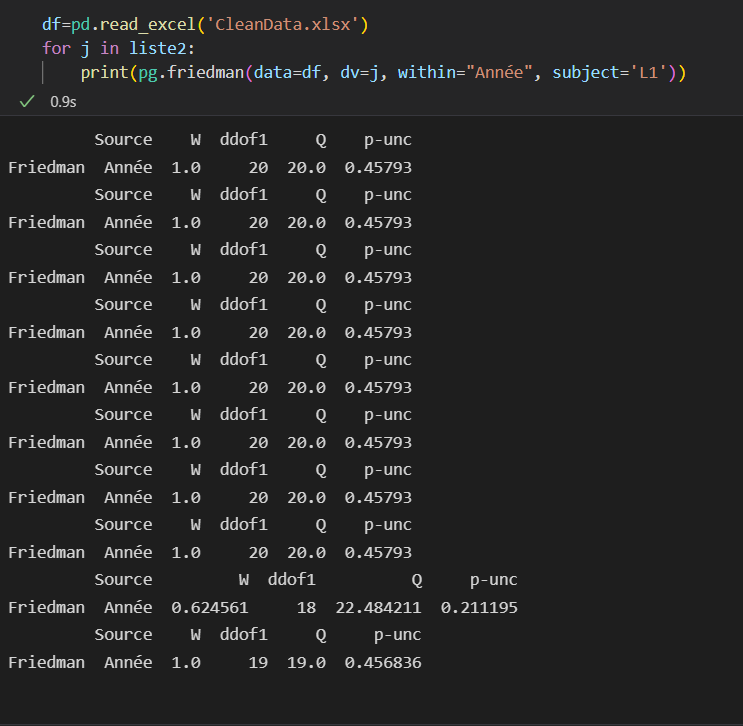
\includegraphics[scale=1]{Images/Friedmann.png}
\\
\bigskip
\\
As seen on the resulst we can say with certitude that years have a huge impact on the different results, but now we have to see if the years of covid are the one who are impacting the most the results.
\bigskip
\\
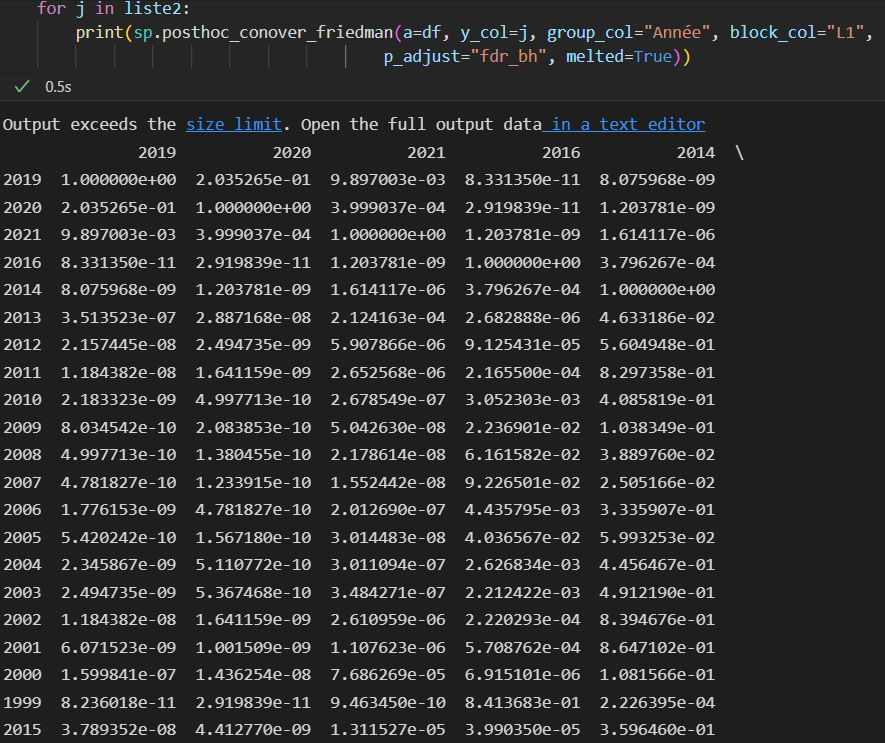
\includegraphics[scale=1]{Images/Friedmann_test.png}
\\
\bigskip
\\
We can see here that most of the variation are between the group of year (2020,2021) and the rest which means the results have indeed been impacted by the covid. We have to check this matrix for every trials and then we will be able to conclude on the impact of covid.
\\



Now we can try again with the gender to know if the covid had a different impact on the results for every gender.


\newpage
\section{\large\bf IV) Conclusion~}
\\
\begin{problem}
In conclusion we can see that the covid had an impact on the students and their physical performances and it had different impact on the women and the men. But because the data that I got were not perfect for example missing two years, or some the results were not exploitable, having to measure exactly how it did can be a bit tricky, since the ANOVA did not work, and the Friedmann can be quite messy to interpret there might be others test which could give more information on the exact impact of the covid.
\end{problem}
\\

\newpage
\section{\large\bf V) Bibliography~}
\\
https://www.python-simple.com/python/statsmodels
\\

https://stackoverflow.com
\\

https://fr.wikipedia.org/wiki/ANOVA/de/Friedman
\\

https://fr.wikipedia.org/wiki/Analyse/de/la/variance
\\

https://www.reneshbedre.com/blog/friedman-test-python.html
\\

\end{document}
